\documentclass[journal]{IEEEtran}
\usepackage[utf8]{inputenc}
\usepackage[table]{xcolor}
\usepackage{tabularx}
\definecolor{tableShade}{gray}{0.9}
\usepackage{graphicx}
\usepackage{caption}
\usepackage{subcaption}
\usepackage{soul}
\usepackage[colorinlistoftodos,prependcaption,textsize=normalsize]{todonotes}
\setlength{\columnsep}{.4cm}
%\documentclass{article}
%\usepackage[utf8]{inputenc}
\usepackage{amsmath}
\usepackage{graphicx}
\usepackage{algorithm2e}
\usepackage{tabularx}

\title{ An Iterative Camera-to-lidar Calibration method using two frames of object points}

\author{\IEEEauthorblockN{
Ju Wong {*}, Venkat R. Dasari{**},  Billy Geerhart {***}, Brian Rapp{***}, Peng Wang{***}}
\\
\IEEEauthorblockA{*}{ Virginia State University, Blacksburg, VA}\\
\IEEEauthorblockA{**}{DEVCOM ARL Army Research Office, Aberdeen Proving Ground, MD 21005}\\
\IEEEauthorblockA{***}{DEVCOM Army Research Laboratory, Aberdeen Proving Ground, MD 21005}
}

\begin{document}

\maketitle

\section{Introduction}

\noindent

There is a growing need for distributed robot systems to share and render 2D and 3D sensory data from different sources in an accurate and consistent manner. This capability is important for performing tasks such as collaborative exploration, mapping,
search and rescue, and data collection. 
In general, multi-robot missions require sensory information to be shared between
the agents for effective operation. Fully autonomous multi-agent
exploration, in particular, requires distributed information sharing in several essential 'backend' tasks: (1) merging of the member robots' sub-maps into a global map, (2) identification and localization of interesting objects, and (3) visualization of 2D and 3D data. To support the above computing tasks, an efficient and robust algorithm to calibrate intra-sensor and inter-sensor parameters is required to correctly integrate data streams from multiple sources. 
Such algorithms,  often implemented as a parametric estimation method, are critical to accurately "superimpose" synchronized data streams such as the camera data and the lidar point cloud.

A promising method to superimpose different sensor data is the diffusion technique \cite{wang2019ldls}, which applies rigid transformations between sensors to obtain an initial alignment, and then uses inherent local features to fine-tune the associations between the raw data. 
Many diffusion algorithms depend on an accurate camera-lidar transformation model. This raises a potential issue: slight errors in the transformation matrix can result in significant mislabeling of the sensor data, as we will show in Section 2. One widely-used remedy is to perform constant re-calibration of the sensor TF matrix to minimize alignment-induced errors. To alleviate the need for frequent re-calibration and reduce the impact of the calibration error, we propose a self-calibration method that allows the robot to estimate the transform (TF) matrix with minimum human involvement and setup requirement. The inter-sensor calibration process typically estimates 6D relative pose or the equivalent transformation matrix between two sensors that are rigidly mounted. In our case, we use the lidar sensor and the camera sensor.

Our lidar-camera calibration method is an iterative search process that minimizes the 3D association error of the observed object at two observation events.
The problem can be formulated as a bundle adjustment problem between discrete time camera data and lidar data from the same robot. 
We found that two LIDAR observations allow us to estimate the relative pose change of the robot using point cloud matching algorithms such as floam \cite{ Zhang-2014-7903} and GICP \cite{gicp}, assuming moderate robot movement. Vice versa, this method can also be used to estimate the position change of a moving object and to segment the moving objects from the background in 3D domains.  Together with the object pixels in the image plane, the estimation of the transformation parameters can thus be solved by finding the optimum 2D-to-3D correspondence of the target object. 
 
Following these observations, our calibration method is summarized below:
\begin{enumerate}
    \item Perform two observations of the dominant object separated by a movement displacement ($\Delta P, \Delta yaw$)
    \item Compute the corresponding lidar points P(0) and P(1)
    \item Compute the closet 2D image plane points from P(k)
    \item Compute a new $[T|R]$ matrix based on current point correspondence
    \item Apply the new transform to get the projected image points P(k+1)
    \item Repeat the above steps until convergence
 \end{enumerate}

 
We evaluated the proposed method using field experimental data collected by a fully loaded Clearpath Jackal robot. Our implementation and computing pipeline is optimized to achieve real-time performance on resource-constrained edge computing autonomous platforms, e.g., unmanned ground vehicles (UGVs).

\section{Related Work}
The lidar-camera calibration is closely related to the classic Perspective-n-Point problems \cite{horn87, low91, quan99}. 
Camera pose estimation \cite{horn87}, also referred to as view point recover problem \cite{low91}, uses 2D-3D correspondence to establish a transformation matrix between 3D observation and 2D observations. The three point P3P case and the four point P4P case, close-form solution can be obtained \cite{horn87}. For $n>4$, the problem must be solved via numerical methods. High accuracy correspondence between the 2D pixels and the 3D points perceived by the robot is essential to build high-level understanding of the world and reasoning in a symbolic world model. 

A closely related problem is to estimate rigid motion using two sets of 3D point clouds. Since Besl's seminal ICP paper \cite{icp}, there is a rich collection of improvements in recent decades \cite{gicp}, especially with the availability of high-resolution 360-degree lidar sensors. The main idea in ICP and its variant is to gradually recompute the point correspondence in such a way that a better transformation matrix can be computed. Our method borrows a similar strategy to assure the convergence of the solution.

The recent effort in this line of work is to use a deep neural network to build point correspondence. The problem however remains a significant challenge. In the 2D domain,
Object detection and segmentation using 2D images
have seen high-accurate solutions through the publication of deep
convolutional neural networks models \cite{ssd,mrcnn}.

In the 3D domain, there are fewer results due to many notable difficulties associated with the 3D point representation and sensor data. For one, the processing of 3D points is much less efficient than its 2D sibling due to its sparseness and wider dynamic range. The 3D point clouds are unstructured by nature
and laborious to label, which results in less availability of training data. Recently there are some promising methods that have demonstrated the feasibility of converting point clouds as input for deep
networks \cite{wu2017squeezeseg},

Our work is also inspired by the LDLS method \cite{wang2019ldls}. The LDLS method uses an Mask-RCNN \cite{mrcnn} to
detect object classes and instances at the pixel level.
The author demonstrates that the 2D label can be diffused to the 3D domain by repeatedly applying a connectivity matrix to the 2D labeling, which can be executed in a GPU with much-improved computing time. The LDLS method
leverages the success of convolutional neural networks for 2D
image segmentation, However, LDLS shows high segmentation error if lidar-camera calibration is not accurate. The error is particularly noticeable near the edge of objects where they board with background or occlude with other objects. 

A key assumption in LDLS and other similar methods is that calibration parameters between the 2D and 3D sensors are well-established. Our contribution is the development of a semi-automatic method that allows the calibration to be done in a much unrestrictive environment by taking advantage of the 2D and 3D observations that are already available at the robot platform.

\section{Problem Formulation}
\subsection{Calibration Parameter Estimation}
The input to the PnP problem consists of a 3D point set $P$ observed in the world frame and the corresponding image point set $I$ observed in the camera image plane, and the solution is a rigid transformation from the world frame to the camera frame, A major difference in our problem setting is that we don't have the 2D-3D point correspondence information. Our method boils down to a novel method to obtain the 2D-3D correspondence, after which the problem can be easily solved using the existing PnP methods.
Before diving into our method, it is necessary to establish some commonly used notations. Let $P_w$ be the point set in 3D world frame, $P_c $ be the coordinate at the camera frame, and $I_o$ the projected pixel set in the image plane, the general calibration process is formulated as a non-linear optimization problem where we minimize the average corner errors. Essentially, we optimize
\[ argmin_{T,R}{\sum_{p \in P}{||d(TR(p), I_o)||}}\] where $TR(p) $ is transformed coordinate of $p\in P_w$  under given calibration parameters $TR$, and $d(p, A)$ is the distance of $p$ to a 2D point set.

The parameter set to be estimated is the transformation matrix $[T | R]$. We assume that the camera projection matrix $M$ is known. 
 \[$M$=\begin{bmatrix}  
    $f_x$ & $0.0$ &  $x_0$  \\
        0.0 & $f_y$ &  $y_0$ \\
       0.0 & 0.0 &  1.0
       \end{bmatrix}\]
       
The 3D transformation matrix $TR_{lc} = [R~| T]$ is break to two parts: $R$ is a 3x3 rotation matrix and $T$ is a 3x1 vector for translational offsets. 
%the Translation vector  [0, -.063, -.267] is the origin of the lidar frame in the camera frame, this is in agreement with the sensor setup. i.e., lidar is 0.267 meters behind the camera, but camera's z-axis car's x-axis (length)

To estimate the calibration matrix TR, we can use a gradient-based search method that minimizes a hand-crafted error function, or we can try to establish the association between the 2D and 3D points and then apply the Perspective-and-Point RANSAC method (PNPRANSAC). We will discuss the later methods. Both methods assume that the object point cloud is separated from the background, which is discussed later in this section.
\begin{table}
    \caption{Symbols definition}
    \label{mysymbls}
        \begin{tabularx}{0.9\textwidth}{l | r}
%        \toprule
%        \midrule
        $P_o(t)$ & Object Point cloud (PC) at $t$ in  body frame  \\
        $P_l(t)$ & True PC at $t$  in robot lidar frame  \\
        $P_c(t)$ & True PC at $t$  in robot camera frame  \\
        $\bar{s}=(x,y,z \bar{q}) $ & object position and quaternion in lidar frame \\
%        \toprule
%        \midrule
         $I_o(t)$ & Object 2D image at $t$  \\
        $\hat{P_o^*(t)}$ & predicted Object PC at $t$  \\
        $TR_c$  &  TF matrix to cam frame & $TM$ &  2D cam proj matrix \\
%          \bottomrule
\end{tabularx}
\end{table}

The relationship between the 2D image data and the 3D lidar data is established first:
\begin{equation}\label{eq:i0}
I_o(t0) = M T_c P_o (to) 
\end{equation}

\begin{equation}\label{eq:i1}
I_o(t1) = M T_c P_o (t1) 
\end{equation}

\begin{eqnarray}\label{eq:i1}
IOU = \frac{P_o(t0) \bigcap P_o(t1)}{P_o(t0) \bigcup P_o(t1)} \\
P_o^*(t0) = T_c^{-1} M^{-1} I_o(t0) \\
\hat{P_o(t0)} = (T_c + T_\delta)^{-1} M^{-1} I_o(t0)
\end{eqnarray}
\begin{figure}[]
    \centering
    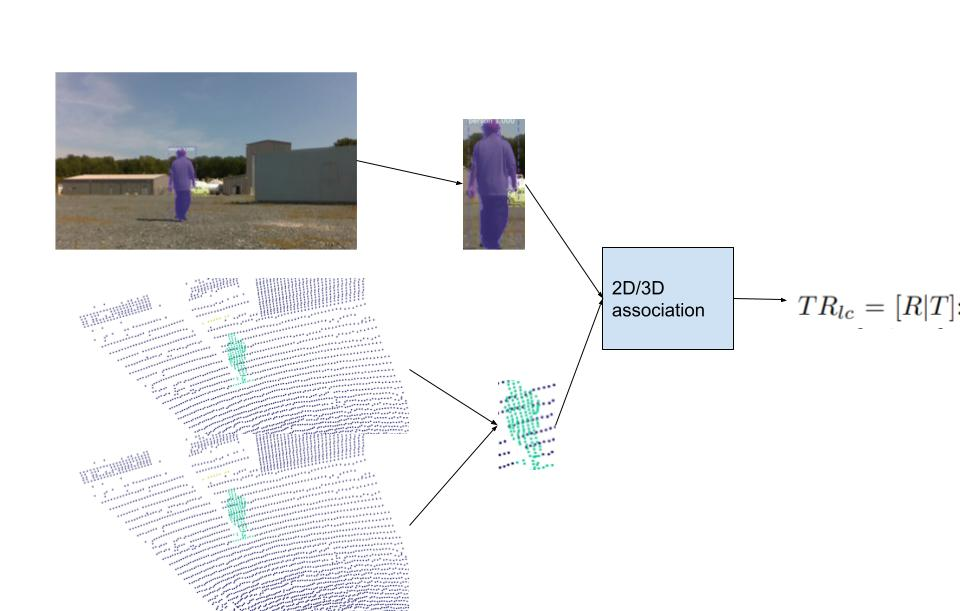
\includegraphics[width=\columnwidth]{images/computing_flowchat.jpg}
    \caption{Computing flowchart for TR matrix estimation via 2D-3D bundle adjustment}
    \label{fig:framework}
\end{figure}  

\subsection{method \#1: 2D keypoints matching followed by PNP}
Existing calibration methods typically require two pattern templates of known geometry features (such as a checkerboard) to establish the correspondence of the keypoints in 3D space and 2D image plane. Our first method also tries to identify 2D keypoints to establish the 2D-3D correspondence. In this method, we first separate the object point cloud $P_l(t0)$ as discussed in section 3.5. We then calculate the projected object footprint using the initial $TR_0$ 
\begin{eqnarray}
    \hat{I(t0)} = TR_0 (P_L(t0))
\end{eqnarray}

If the initial value $TR_0$ is close enough to the optimal solution, it can be expected that 
$\hat{I(t0)}$ and the actual $I(t0)$ will been nearly identical subject to an affine transformation. In particular, we can extract keypoints from $\hat{I(t0)}$ and $I(t1)$ and establish their association using a feature extractor such as SIFT. Let $Key(I(t0)) $ and $Key(\hat{I(t1)}) $ be the respective keypoints extracted. We now have a set of associations between the 2D key points $Key(I(t0)) $ and their corresponding 3D counterparts. The least-square error solution $TR_{lc} $ can be readily obtained by applying a PnP solver such as Lu's gradient search method \cite{lu}

Assuming moderate object movement, it is expected that the delta should remain a very small portion of the object PT. 

\subsection{method \#2: Closest 2D point Matching}
In this method, instead of using image domain features to calculate a set of key points as 2D-3D corresponding pairs, we iteratively estimate the 2D-3D correspondence for all observed 3D points. We use a similar strategy as the one used in ICP \cite{icp} to compute two quantities iteratively: a candidate 3D-2D point correspondence, and the 3D-2D transformation parameters estimated using PnP. At each iteration, we use a $Closest()$ operator to predict the subset of the image pixels that are most likely to be the true projection. The resultant pixel set in turn allow a new TR matrix to be computed which move closer to the optimal TR. Intuitively, the reason this might work is exactly the same as the case of ICP algorithm. 

\begin{algorithm}[!htbp]
	\caption{Iterative Calibration Parameter Search}
	\label{alg:model}
	\SetKwProg{Function}{Function}{}{end}
    \SetKwFunction{AL}{CaliberationOptimizer}
	\SetKwFunction{Proj}{Projection}
    \SetKwFunction{Sense}{CollectSensorData}
    \SetKwFunction{Closest}{Closest}
    \SetKwFunction{GoodModel}{MeetUserRequirement}
    \SetKwFunction{PnPsolver}{PnPsolver}
    \SetKwFunction{Apply}{Apply}
    \KwIn{\\%
        \qquad $PC_0, PC_1$: point clouds at two time inst; \\
        \qquard $~~I_0, I_1$: 2D object mask segmentation ;
        \qquad $TR_0$: initial calib matrix;}
    \KwOut{\\%
        \qquad $TR_n$: final calib matrix;\\}

    \Function{\AL}{
        \tcc{Extract object points from PC_0, PC_1}
        ($\hat{P_0}$, $P_1$) $\gets$ \ObjExtract($PC_0$, $PC_1$) \\
        \tcc{Calculate 2D Projection of P_0, P_1}
        ($\hat{I_0}$, $C_0$) $\gets$ \Proj($TR_0$, $P_0$) \\
        \tcc{Build 2D-3D correspondence iteratively }
        \For{$i \in (0, 1, 2, \ldots)$}{
            $I_k $ $\gets$ \Closest($\hat{I_0}$, $I_{k-1})$ \\
            \tcc{Computer the new TR}
            ($TR_{k,i}) $\gets$ \PnPsolver($P_0, I_k$)\\
            \Apply($TR_{k}, P_0$))\\
            $T_{i+1}$ \gets $T_i \cup S_{t,i}$ 
       }
    }
\end{algorithm}

Here again, we emphasize that $P_{0/1}$ is the estimated 3D point cloud 
of the target object and not the whole-scene point cloud. This is important to assure the convergence of the algorithm since the $Closest()$ operation is only meaningful when the projected pixel set and the observed object pixel set "mostly" belong to the same object. 

\subsection{Separation of object point cloud and relative pose estimation}
We now discuss the separation of the target object from the background and nearby objects of the two point clouds. The ground plane and static structure are processed separately. 

We first prune the point cloud with a camera view model such that the remaining points will only contain one moving object and static background. This is a reasonable assumption in caliberation scenario. The inview cut is necessary to remove points corresponding to the human objects, which typically stand behind the robot. The inview cut allows us to remove 70\% of lidar points.
It is expected that the delta should remain a very small portion of the object PT. 
The relative pose estimation method:

(1) GICP to get delta pose of the observing object
(2) get $\hat{P}$ from $I(t)$

After the above processing, the size of the point set has about 300 points when the target object (a jackal robot) is about 4 meter in front of the observing robot. Figure \ref{fig:objext} shows the extracted point sets at two time instances.

\begin{figure}[]
    \centering
    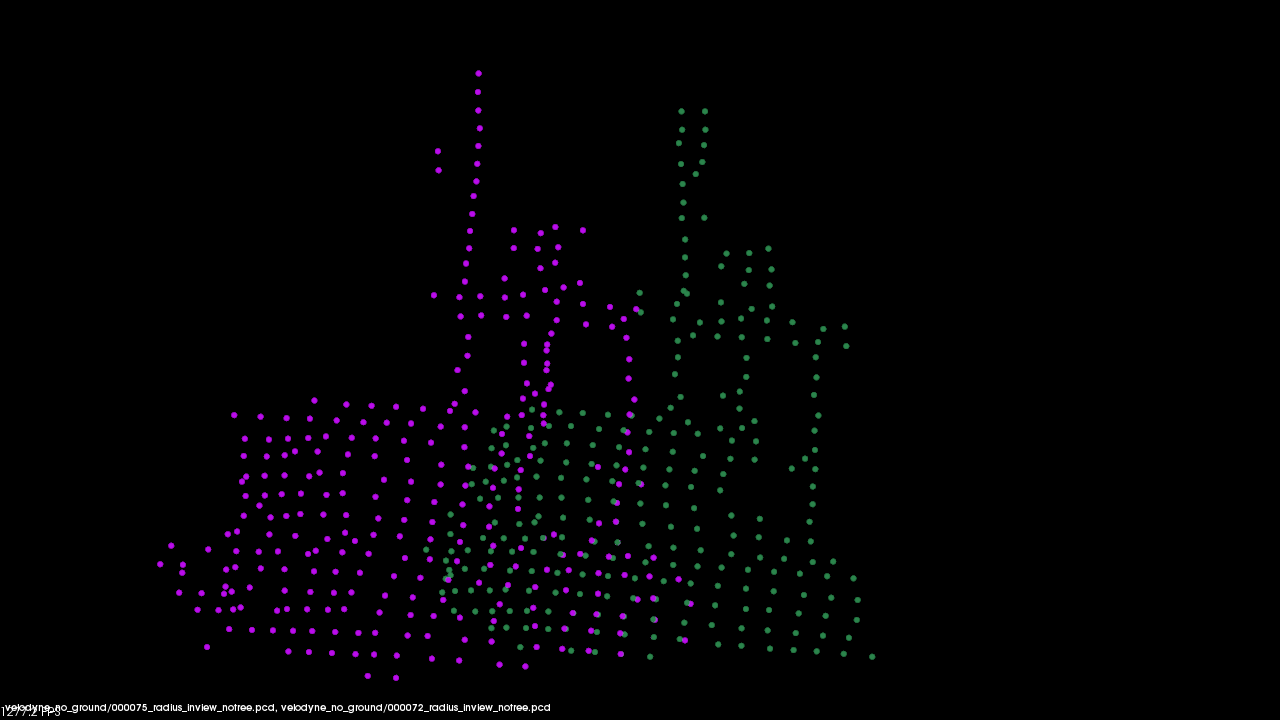
\includegraphics[width=0.5\columnwidth]{images/obj_072_075.png}
    \caption{Object point clouds overlayed}
    \label{fig:objext}
\end{figure} 
\begin{figure}[]
    \centering
    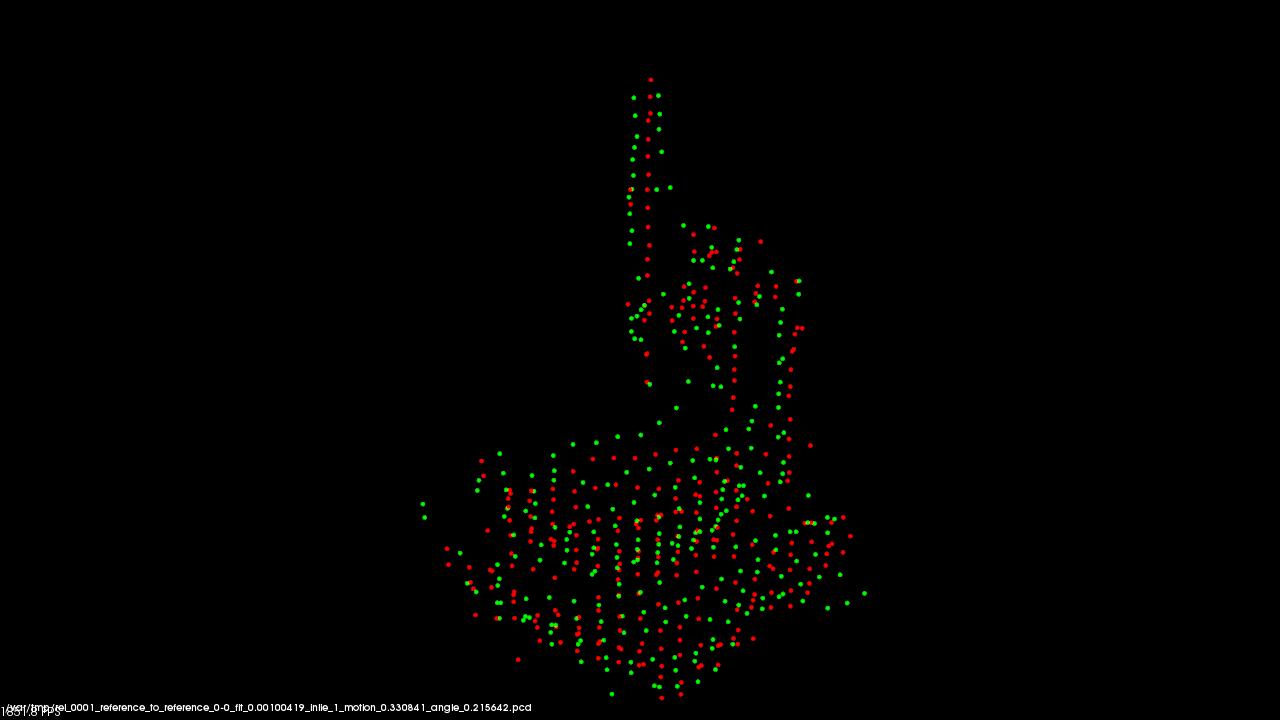
\includegraphics[width=0.5\columnwidth]{images/gicp_072_075.png}
    \caption{GICP matched Object point clouds}
    \label{fig:gicp_result}
\end{figure} 

\subsection{2D Closest matching }
The remaining task is to build a 2D-2D matching between the projected 2D coordinates and the image pixels of the observed object points by the camera, i.e., a mapping function $g(\hat{I}) \rightarrow I_o$ that map a purple points to a green points in figure \ref{fig:objext}. Noticing that the shape of the projected object points is largely preserved,  
we opt to use a simple three-parameters linear transformation to approximate $g()$: we first find the centroids for both pixel sets $c_0$ and $c_1$, we then calculate the dominant axis at each centroids, $\overrightarrow{x_0}$, $x_1$, and the associated perpendicular axis $\overrightarrow{x_0}$, $x_1$. From which the scale factors on the two axis can be calculated as $s_0, s_1$, as well as a rotational parameter $\theta$. The mapping in 2D image plane is now defined as:
\begin{eqnarray}
(\hat{u_0}, \hat{v_0})^T = [s0, s1] R_{\theta} (u_1, v_1) \\
(u_0^*, v_0^*) \in I_0 ~ minimize |(\hat{u_0}, \hat{v_0})^T, I_0)|
\end{eqnarray}

\begin{figure}[]
    \centering
    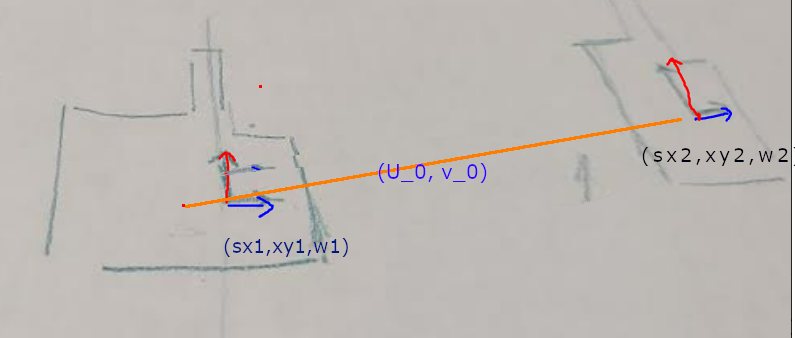
\includegraphics[width=0.5\columnwidth]{images/2dpoints_match.png}
    \caption{2D projection matching using simple max/min scaling and rotation}
    \label{fig:gicp_result}
\end{figure} 
\section{Evaluation}
We can calculate the IOU index for the interested objects/landmarks, which allows us to evaluate how close a TF matrix is to the ground truth, Assuming the observed object (such as a human figure, or a vehicle) appears in both the Lidar data and the camera data at two separate time instances $T_0$ and $T_1$. We can thus calculate the corresponding lidar points $P(t_0)$ of the landmark and  $P(t_1)$. Assuming that the observer (robot) moves a small displacement from $T_0$ to $T_1$, One would expect a high IOU $\frac{P(t_0) \cap P(t_1)}{P(t_0) \bigcap \cup P(t_1)}$ if the initial transformation matrix is accurate. If the IOU is low, one might suspect that the initial transformation parameters are no longer correct.

\begin{figure}[]
    \centering
    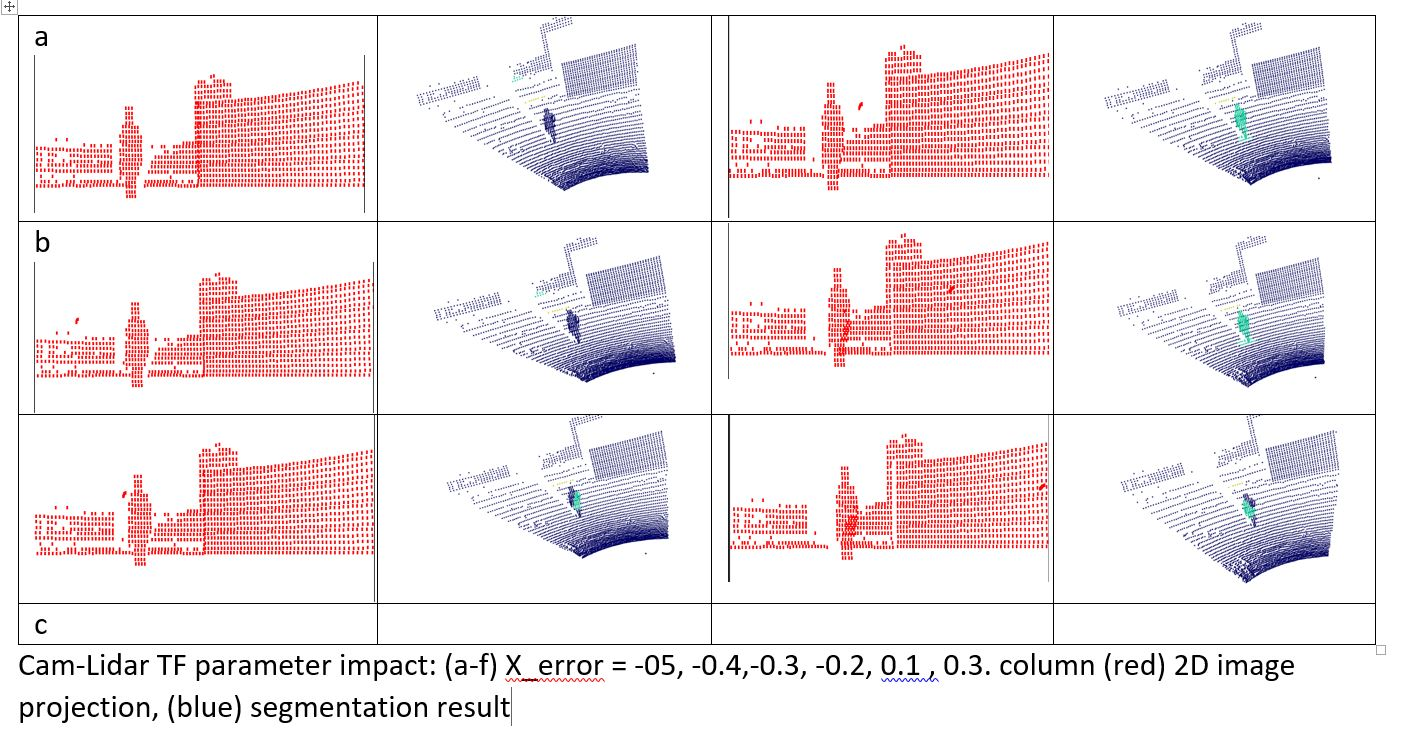
\includegraphics[width=0.5\columnwidth]{images/figure3.JPG}
    \caption{}
    \label{fig:framework}
\end{figure}   


\section{Conclusions}

\bibliographystyle{IEEEtran}
\bibliography{references} % bibliography data in report.bib

\end{document}
